\section{Introduction}

\begin{frame}{Basic motivation}
  \centering
  Binary analysis requires \alert{\gls{cfg} reconstruction}%
  \vfill
  \begin{tikzpicture}[every node/.style={draw,ellipse},->]
    \node (x) {$x$};
    \node[below=1cm] (5) {5};

    \draw (x) -- (5) node[midway, right, draw=none] {\inlineasm{jmp 5}};
  \end{tikzpicture}
\end{frame}

\begin{frame}{Problem}
  \centering
  \Gls{cfg} reconstruction is \alert{undecidable} due to \alert{indirection}%
  \vfill
  \begin{tikzpicture}[every node/.style={draw,ellipse},->]
    \node (x) {$x$};
    \node[below=1cm] (where) {?};

    \draw (x) -- (where) node[midway, right, draw=none] {\inlineasm{jmp rax}};
  \end{tikzpicture}
\end{frame}

\begin{frame}{Even worse}
  \centering
  \alert{Exceptional control flow} increases complexity!%
  \vfill
  \begin{tikzpicture}[every node/.style={draw,ellipse},->]
    \node (x) {$x$};
    \node[below right=1cm of x] (where) {?};
    \node[below left=1cm of x] (except) {???};

    \draw (x) -- (where) node[near start, right, draw=none] {\inlineasm{jmp rax}};
    \draw[dashed] (x) -- (except);
  \end{tikzpicture}
\end{frame}

\begin{frame}{And\dots\hspace{.5cm}
    
\includegraphics[height=.75cm]{GHIDRA_1}\hspace{.5cm}
    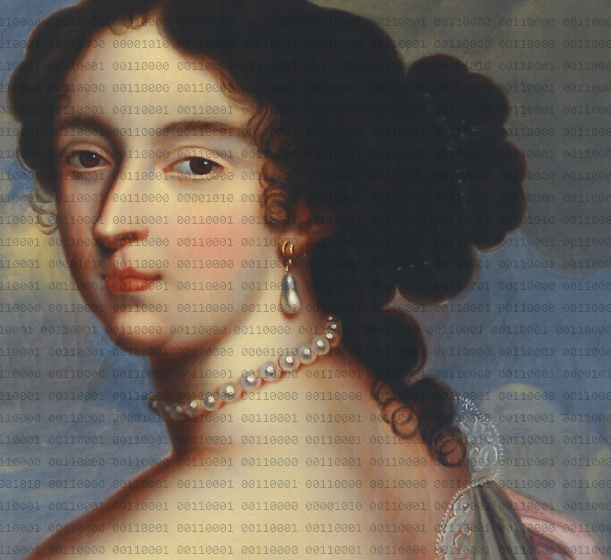
\includegraphics[height=.75cm]{ida}\hspace{.5cm}
    
\includegraphics[height=.75cm]{ninja}
  }{existing binary analysis tools do not model it!}
  \centering
  \only<1>{
  \tikzstyle{landing}=[draw=none,text opacity=0]
  \tikzstyle{unwind}=[draw=none]
  \tikzstyle{regular}=[->]
  }
  \only<-2>{\tikzstyle{good}=[]}
  \only<-3>{\tikzstyle{bad}=[]}
  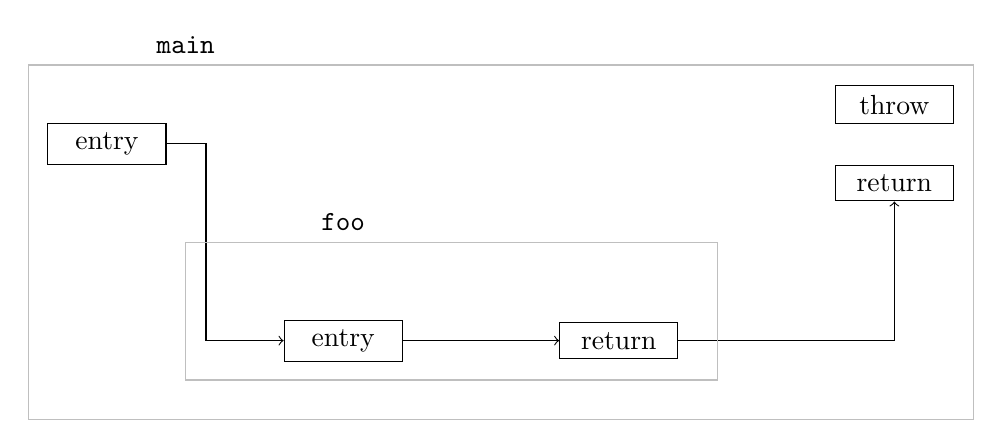
\begin{tikzpicture}[y=-1cm, minimum width=1.5cm, every node/.style=draw]
    \node[draw=none] (main) at (1,-0.75) {\texttt{main}};
    \node (mainE) at (0,0.5) {entry};
    \node[good] (mainR) at (10,1) {return};
    \node[bad] (mainT) at (10,0) {throw};
    \node[landing] (mainLP) at (8,0) {LP};

    \node[draw=none] (foo) at (3,1.5) {\texttt{foo}};
    \node (fooE) at (3,3.0) {entry};
    \node[good] (fooR) at (6.5,3.0) {return};
    \node[landing] (fooLP) at (5.5,2.25) {LP};

    \draw[regular] (mainE.east) -- ([xshift=0.5cm]mainE.east) |- (fooE.west);
    \draw[regular] (fooE.east) -- (fooR.west);
    \draw[regular] (fooR.east) -- (fooR.east -| mainR.south) -- (mainR.south);

    \draw[unwind] ([yshift=0.15cm]fooE.east) -- ([xshift=0.5cm,yshift=0.15cm]fooE.east) |- (fooLP.west);
    \draw[unwind] (fooLP.east) -- ([xshift=0.5cm]fooLP.east) |- (mainLP.west);
    \draw[unwind] (mainLP.south) -- (mainLP.south |- mainR.west) |- (mainR.west);
    \draw[unwind] (mainLP.east) -- (mainT.west);

    \draw[lightgray] (1,1.75) rectangle (7.75,3.5);
    \draw[lightgray] (-1,-0.5) rectangle (11,4);
  \end{tikzpicture}%
  \vfill
  \begin{tabular}{rl}
    \uncover<2->{Dashes                         & \alert{unwinding} edges \\}
    \uncover<3->{\textcolor{green}{Green boxes} & regular return \\}
    \uncover<4->{\textcolor{red}{Red box}     & exceptional termination}
  \end{tabular}
\end{frame}
